%===================================== CHAP 3 =================================

\chapter{Simulator for 360 degree fisheye lens image capture on an UAV} \label{chap:simulator}

This chapter shows the implementation of a calibratable camera simulator for capturing omnidirectional fisheye lens images in Unreal Engine, building upon an already existing robotics simulator plugin called AirSim\footnote{github.com/Microsoft/AirSim} \cite{Airsim_paper}. The existing simulator is augmented with a ROS\footnote{ros.org/} interface, an omnidirectional camera model with modeled fisheye lens distortion, and the ability to transform and combine the perspective pictures captured into a single wide-angle fisheye lens-distorted image. For now, the simulator will only support the fourth order polynomial distortion model, shown in Table~\ref{tab:theory_fisheye_lens_model}.

The chapter is split into two parts. The first sections will show related work on camera simulators for robotics and current advancements in the field, as well as discuss relevant platforms to base the omnidirectional camera simulator on. The second part will go deeper into the implementation of the simulator itself, with a focus on the augmentations done within the scope of this project.

\section{Related work} \label{sec:simulator_related}

As mentioned in Section~\ref{chap:introduction}, there has been a lot of recent development within the area of computer vision for use with UAVs, which has produced the need for realistic simulators to ease the testing process, decrease costs and increase the efficiency. Some simulators are built from the ground up, like V-REP \cite{VREP2013} and Gazebo \cite{GazeboPaper}. While these are general purpose robotics simulators, there are multiple projects extending these simulators to connect to other interfaces or concentrate on specific tasks. RotorS\footnote{github.com/ethz-asl/rotors\_simulator}~\cite{RotorS} is an example of such a simulator, focusing on control and state estimation for MAVs. This simulator is built on top of Gazebo and Gazebo's ROS interface, adding MAV and Sensor models, while extending Gazebos capabilities for MAV control and state estimation.

Since 2010 there has been an increase in the use of game engines and other graphically capable software to help increase the realism of computer vision simulators. HNMSim \cite{HNMSimPaper} is made for simulating networks for UAVs. It combines the use of MATLAB, Simulink, and LabView, with the game engine Unreal Engine and 3D modeling software Autodesk 3Ds Max, to create more realistic environments for the simulations. They also implemented and simulated a multirotor with an attached camera in Unreal Engine. Another similar simulator\cite{UnityROSsim} built upon the Unity game engine, implemented a multirotor and a Lidar model with ROS as the external interface for control algorithms.

In 2017, two simulators for simulating autonomous vehicles in realistic environments were released: Sim4CV \cite{Sim4CV_paper} and AirSim \cite{Airsim_paper}. Both implement a multirotor and a car model, using Unreal Engine as their original backend. It should be mentioned that in late 2018, Microsoft started developing AirSim for Unity as well, and it looks like they will support both engines going forward. Both of these will be discussed in more detail in Section~\ref{sec: UnityUnreal} and \ref{sec:Chooseplatform}.

While experiments have been done using real or synthetic datasets showing that it can be beneficial to use fisheye or catadioptric cameras over perspective cameras for some applications \cite{Zhang2016BenefitOL, OmniVIOKalman, CompOmniVSLAM}, there are no released open source simulators for $360^\circ$ camera captures with the possibility for closed loop operation. One probable reason for this is that only perspective camera models have been implemented in most simulators. There was a promising looking project implementing a $360^\circ$ fisheye camera for Gazebo shown as a tutorial at Gazebo's tutorials page \cite{GazeboWideWeb}. However, this seems to have been removed recently, as it is no longer available. Both Unity and Unreal Engine on the other hand support capturing scenes to cube maps. Cube maps are made of 6 images with a common focal point for their projection, covering all directions in the scene. This has been used to capture $360^\circ$ video, as seen in \cite{UnityCubeCapture, UnrealCubeCapture}. It has, however, not been implemented as a part of either of the simulators mentioned. 

The simulator implemented in this project will be based on a previously developed simulator, and the focus will be on adding a $360^\circ$ camera to work with the already existing framework. Due to a lack of experience with simulators and game engines, there will be a focus on open software, with a sizeable community, which is still used and supported by the developers. Gazebo, Unreal Engine and Unity match these criteria. For this reason, these platforms will be compared as alternatives. An important note is that this should not be treated as a comprehensive comparison of the different simulators or game engines mentioned, and far from all features will be presented. This comparison is a result of the initial research done, in order to make an omnidirectional camera simulator for robotics applications.

\section{Gazebo} \label{sec:Gazebo}

Gazebo is a simulator platform made for robot simulation, with 3D graphics for Linux platforms, and can be built with four different physics engines \cite{Gazebo_phys}. The four engines are optimized for different purposes, making Gazebo quite versatile when it comes to simulations. Gazebo is fully usable as a standalone, but it also comes with native ROS support. This means that project specific hardware can be modeled in Gazebo and run the same ROS code as it would have been done with the physical robot.

The simulations in Gazebo are built from XML-files describing the world, models that inhabit the world, and the physical properties of each model. The models can be attached to one another through joints and links to create more complex models. Gazebo also provides the ability to add specific behavior to the simulation through plugins. Plugins are compiled C++ code attached to a specific component, like a model, sensor or world. It is also through these plugins ROS behavior is defined.

The camera sensor implements a perspective camera, giving access to the typical camera parameters: horizontal FoV, image height, image width, color coding, and near and far clipping plane. Gazebo also comes with support for adding Gaussian noise and distortion to the camera. The distortion is based on Brown's distortion model\cite{BrownModel}, which models both radial and tangential distortion effects to the output picture. There are no shutter speed settings, meaning that motion blur and exposure time settings are not naturally supported.

\begin{figure}[!htb]
    \centering
    \begin{subfigure}{0.49\textwidth}
        \centering
        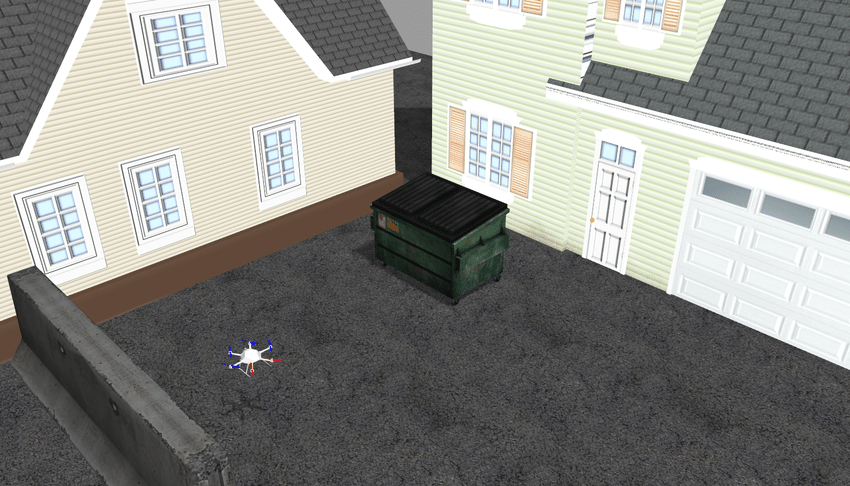
\includegraphics[height=4.25cm]{rapport/fig/Simulator/A-screenshot-of-the-RotorS-simulator-The-scene-is-built-up-from-Gazebo-default-models.png}
        \caption{From RotorS simulator paper \cite{RotorS}.}
        \label{fig:A}
    \end{subfigure}
    \begin{subfigure}{0.49\textwidth}
        \centering
        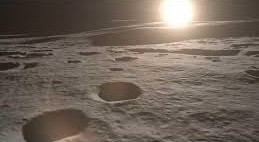
\includegraphics[height=4.25cm]{rapport/fig/Simulator/gazebomoon.jpg}
        \caption{Moon simulation by NASA \cite{NASAGazeboppt}.}
        \label{fig:NASA_Gazebo_moon}
    \end{subfigure}
    \caption{Comparison Gazebo simulations with built-in shader(left) and custom shader(right). The simulation on the right also implements custom imported materials.}
    \label{fig:Gazebo_imgs}
\end{figure}

Another drawback of Gazebo is its graphical capabilities of the built-in model editor. Although meshes and textures may be imported from other 3D modeling software, there are limited ways of editing these inside the editor. This makes it difficult to create realistic scenes. This is especially true when it comes to implementing vegetation and foliage, like grass, trees, and flowers, as these require fine-tuning together with the other elements in the scene to look realistic. The capability of the shader is also quite limited compared to other 3D modeling software, making it hard to create realistic light settings, especially with multiple light sources. There is, however, support for using custom shaders, as NASA did in~\cite{NASAGazeboppt}, showing that it is possible to augment the capabilities of Gazebo to produce good results. Figure~\ref{fig:Gazebo_imgs} shows a comparison between two environments made in Gazebo. The left picture shows an environment from the RotorS simulator, using mostly built-in models and materials, while the right picture shows a custom imported environment with a custom built shader.

\section{Unity and Unreal Engine 4} \label{sec: UnityUnreal}

Unity and Unreal engine are the most popular game engines freely available. Being game engines, both heavily focus on productivity in graphics design, as well as visuals of the final product. This means that a large part of the software toolkit is based around editing the scene and objects in it to look realistic. Both engines provide extensive tools for making custom meshes, textures, animations and lighting effects, making the graphical development of the simulation much easier than in Gazebo. In addition to this both Unity and Unreal Engine provide a large library of premade scenes to use freely, as well as a marketplace where you can buy assets others have made. Figure~\ref{fig:showcase_unityunreal} shows two images of scenes made in Unity and Unreal Engine. Rendering scenes of this quality will require more powerful hardware than what is needed for Gazebo, especially for real-time simulations, but the pictures show the power of the tools provided in these engines. 

\begin{figure}[!htb]
    \centering
    \begin{subfigure}{0.49\textwidth}
        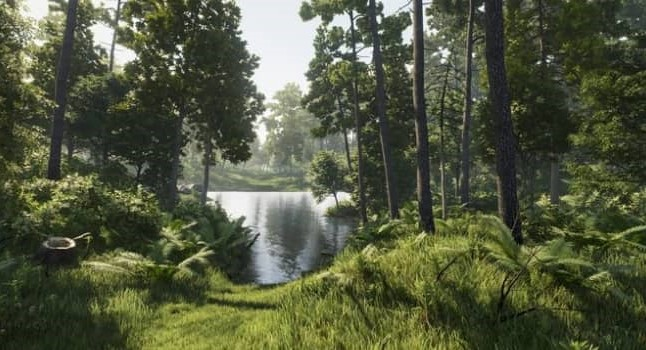
\includegraphics[height=4.2cm]{rapport/fig/Simulator/unrealforest.jpg}
        \caption{Made by Michal Franczak using the Unreal Engine 4 editor \cite{Unrealshowcase}.}
        \label{fig:unreal_forest}
    \end{subfigure}
    \begin{subfigure}{0.49\textwidth}
        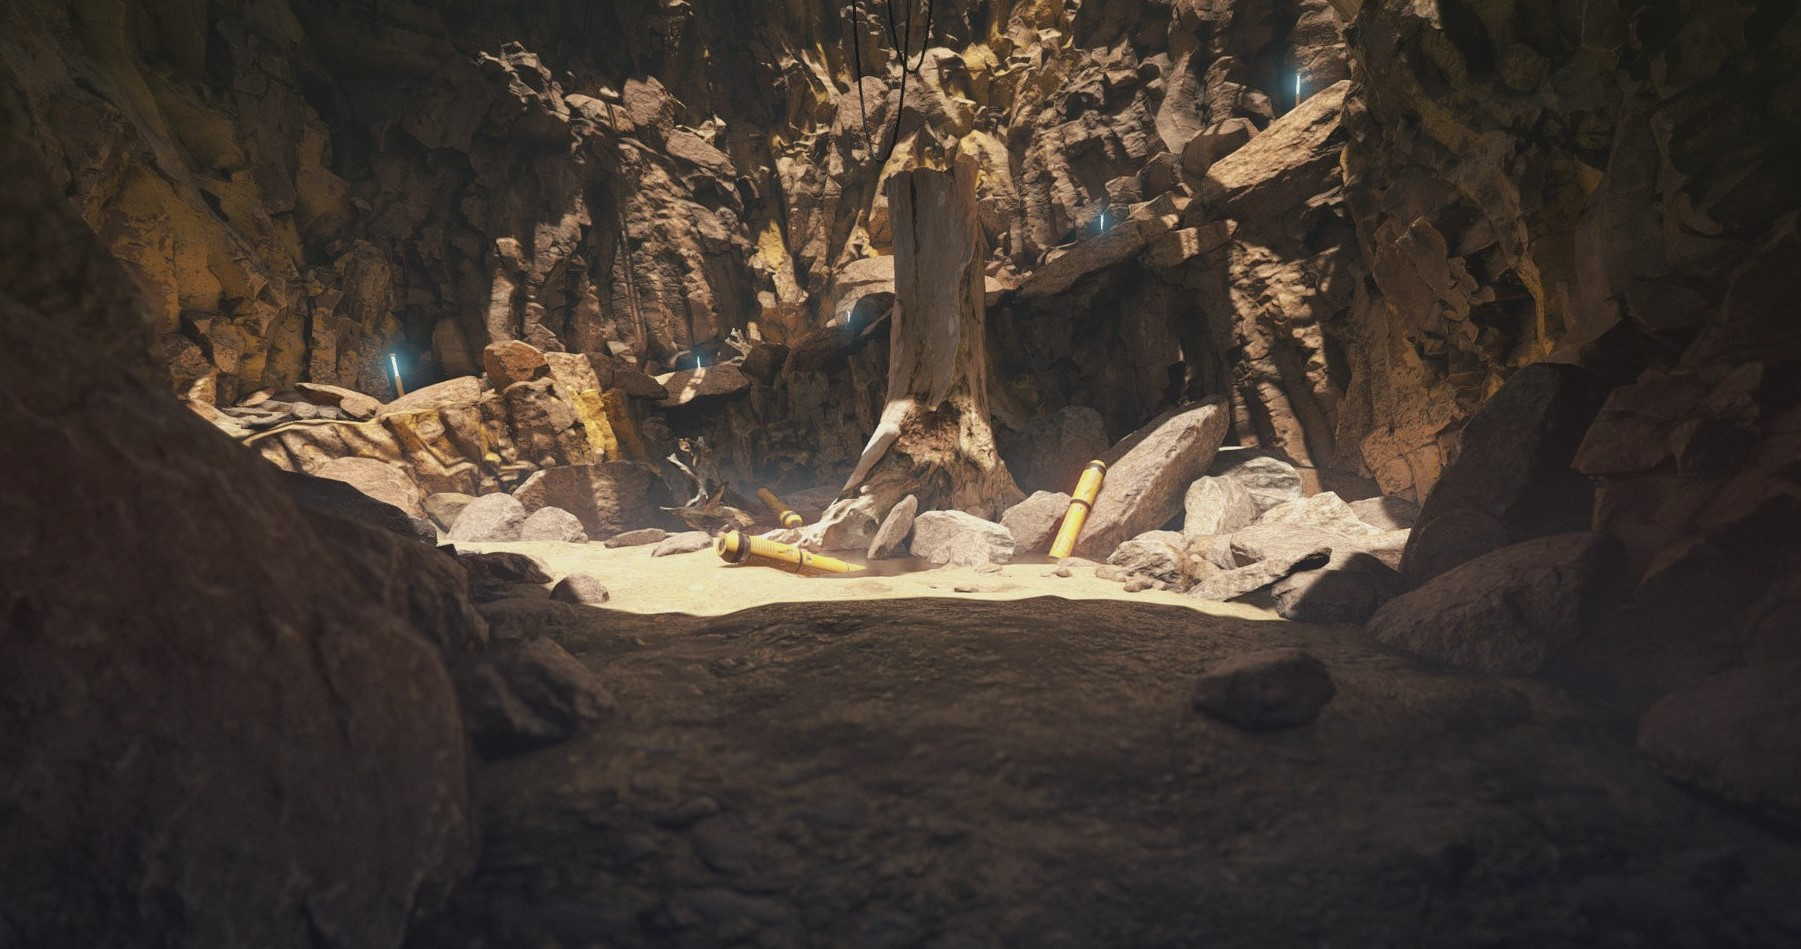
\includegraphics[height=4.2cm]{rapport/fig/Simulator/unitycave.jpg}
        \caption{Created by Pat Goodwin using the Unity editor \cite{Unityshowcase}.}
        \label{fig:Unity_cave}
    \end{subfigure}
    \caption{Showcase of two quite realistic looking environments created in Unreal Engine 4 (left) and Unity (right).}
    \label{fig:showcase_unityunreal}
\end{figure}

Unity is based around the scripting language C\# to change the behavior of the object. The script itself is then attached to a specific object. The behavior is defined through five user-defined functions: $Awake()$, $Start()$, $Update()$, $FixedUpdate()$, and $LateUpdate()$. The $Awake()$ and $Start()$ functions are called once, while the remaining functions are called every frame. Most importantly it is noted that $FixedUpdate()$ is specifically used for updating physics, while $Update()$ is for general purpose updates. However, it is not required to use the provided physics engine.

Unreal Engine is built quite similarly to Unity in regards to the building blocks of the Editor. However, there are two ways to define behavior. One is through C++ and the other is through a visual scripting language called Blueprints. The functionality of Blueprints is almost identical to that of the C\# scripting in Unity. However, the programming interface is graphical and node based, as seen in Figure~\ref{fig:blueprint_editor}. The complete source code of Unreal Engine is freely available, and the user is allowed to make changes to the engine itself. Through registering as an Epic Games developer, access is given to all features of Unreal Engine through the C++ source code. This enables the ability to apply extra optimizations for specific problems, which may be relevant for performance critical tasks. The same interface available to the Blueprints is also available to C++, providing a programming alternative to Blueprints.

\begin{figure}[!htb]
    \centering
    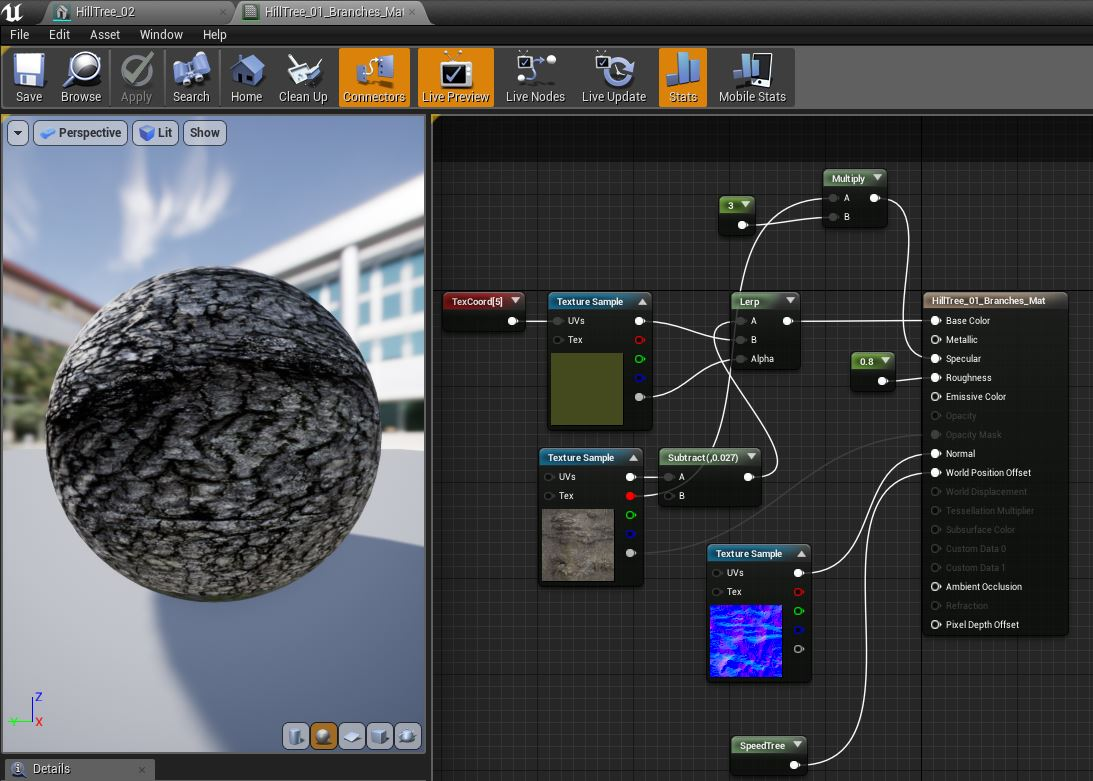
\includegraphics[height = 6cm]{rapport/fig/Simulator/blueprintprog.JPG}
    \caption{Partial picture of UE4 Blueprint for tree branch texture.}
    \label{fig:blueprint_editor}
\end{figure}

The fact that the physics engine is optional is very different from the implementation in Gazebo, where physical properties like mass and inertia are core parts of a model. While the physics engines do implement solvers for collision, interaction through joint and links and physical properties, there is no initial support for simulation of wind or other fluid mechanics.

When it comes to computer vision applications, there is no native support for this in the engines. This may be solved by using OpenCV\footnote{https://opencv.org/} as a part of the project. There exists a wrapper for OpenCV in Unity, and the OpenCV libraries may be linked directly into the Unreal Engine projects through C++ code. OpenCV provides many computer vision algorithms, as well as algorithms for machine learning, and can be used to augment the engine's cameras for wide angle functionality, lens distortions or similar effects. To get an interface to create image datasets from Unreal Engine, a plugin has been created called UnrealCV~\cite{UnrealCV}. This plugin, however, does not support omnidirectional captures or lens models at the moment.

Sim4CV and Airsim both simulators implement a model for a multirotor and a car. While Sim4CV is written directly into Unreal Engine, AirSim is available as a plugin. According to the paper released with Sim4CV, this fact limits the capabilities of the physics simulations of AirSim \cite{Sim4CV_paper}. Since AirSim is implemented as a plugin, it is possible to integrate it with existing projects, and the procedure is well documented in their Github repository. This means that it is relatively easy to integrate AirSim into environments that were not created with AirSim in mind. 

When it comes to interfacing, both simulators implement an application program interface(API) for Python, as well as C++. Sim4CV also implements an API for MATLAB\footnote{www.mathworks.com/products/matlab.html}, which might be useful since MATLAB has lots of CV toolboxes available through the license provided by the Norwegian University of Science and Technology(NTNU). Though none of them directly implements an interface to ROS, there are examples of simple ROS communication with AirSim in their repository.

Though both simulators implement much of the same features, the differences between the two come in the form of their main focus. Sim4CV focuses on computer vision, and the usage of computer vision for machine learning and deep learning, while AirSim mainly focuses on supporting different types of sensors. This means that for projects aiming for sensor fusion, or testing complete vehicle systems, AirSim would be preferred. Sim4CV may, on the other hand, be preferable for AI computer vision projects, especially for deep learning, as it implements a TensorFlow-like interface.

\section{Choosing a platform for the simulator} \label{sec:Chooseplatform}

As mentioned at the beginning of this chapter, the goal of this project is to implement a simulator for capturing realistic $360^\circ$ images with fisheye lenses, with the ability to calibrate the camera parameters to match real fisheye lens cameras. In addition, the simulator should provide an interface to ROS, to enable the simulator to be used with already existing implementations of SLAM and VO algorithms for ROS. This criterion limits the usage to Linux based systems, as ROS is currently only available on Linux platforms. While Unity and Unreal Engine are most optimized for development on Windows or Mac OS, both provide the ability to build their latest releases on Linux. Table~\ref{tab:comparison_interface} shows a comparison of the interfaces of Gazebo, Unity and Unreal Engine.

\begin{table}[!htb]
    \centering
    \caption{Interface comparison of Gazebo, Unity and Unreal Engine.}
    \label{tab:comparison_interface}
    \begin{tabular}{|c|>{\centering\arraybackslash}m{2cm}|>{\centering\arraybackslash}m{2cm}|>{\centering\arraybackslash}m{2.8cm}|>{\centering\arraybackslash}m{2cm}|>{\centering\arraybackslash}m{2cm}|>{\centering\arraybackslash}m{2cm}|>{\centering\arraybackslash}m{2cm}|} \hline
        \textbf{Software}          & \textbf{OS}  & \textbf{ROS} & \textbf{Model/Scene toolbox}   & \textbf{Sensor models} & \textbf{Language}              \\ \hline \hline
        Gazebo          & Linux           & Yes           & Simple  & Yes & C++, XML                 \\ \hline
        Unity           & Windows, Mac OS, Linux                    & No            & Extensive & Plugins & C\# \\ \hline
        Unreal Engine   & Windows, Mac OS, Linux  & No            & Extensive & Plugins/ custom versions & C++, Blueprint \\ \hline
    \end{tabular}
\end{table}

The main advantages Gazebo has over the game engines is its implementation of multiple physics engines, its ROS integration, and its modular sensor setup. A large part of the community also uses Gazebo for computer vision purposes, which may provide more useful help online for the project. The main drawback of Gazebo is that there is limited tooling for graphical development. This means that there are relatively few high-quality scenes made for Gazebo. Making these from scratch would require much more time and experience, as well as additional graphical software, which is unreasonable for the scope of this project. 

The tools available in the Unreal Engine and Unity, provide a much easier way to make high-quality scenes for a camera, or editing scenes that are readily available. The fact that both of these engines also support omnidirectional video capture through cube maps may be helpful when implementing the $360^\circ$ camera feature. The main advantages of Unity and Unreal Engine are their advanced shader and post-processing unit, which can capture multiple effects seen in normal cameras, like motion blur caused by the combination of slow shutter speed and movement. In Table~\ref{tab:comparison_camera} it can be seen that Gazebo has the most advanced distortion model. This is true even with the extra functionality provided by AirSim and Sim4CV. For this reason, additional post-processing of the images must be applied to the images, to obtain the same distortion effects.

\begin{table}[!htb]
    \centering
    \caption{Camera comparison of Gazebo, Unity and Unreal Engine.}
    \label{tab:comparison_camera}
    \begin{tabular}{|c|>{\centering\arraybackslash}m{3.5cm}|>{\centering\arraybackslash}m{3.7cm}|>{\centering\arraybackslash}m{4cm}|} \hline
        \textbf{Camera} & \textbf{Gazebo} & \textbf{Unity} & \textbf{Unreal Engine} \\ \hline\hline
        Camera type     & Perspective & Perspective, Cubemaps & Perspective, Cubemaps \\ \hline
        Distortion model & Radial, Tangetial & Radial, Post-processing  & Post-processing, "Panini Distortion"\cite{panini} \\ \hline
        Noise           & Yes & Yes & Yes \\ \hline
        Exposure time   & No & Yes & Yes \\ \hline
        Motion Blur     & No & Yes & Yes \\ \hline
        
    \end{tabular}
\end{table}

\begin{table}[!htb]
    \centering
    \caption{Built-in shader capabilities of Gazebo, Unity and Unreal Engine.}
    \label{tab:comparison_shader}
    \begin{tabular}{|>{\centering\arraybackslash}m{3cm}|>{\centering\arraybackslash}m{3.5cm}|>{\centering\arraybackslash}m{4cm}|>{\centering\arraybackslash}m{3.5cm}|} \hline
        \textbf{Shader effects} & \textbf{Gazebo} & \textbf{Unity} & \textbf{Unreal Engine} \\ \hline\hline
        Light types     & Lightmaps, Spot, Directional, Point, Ambient & Lightmaps, Spot, Directional, Point, Area, Ambient, Fluorescent & Same as Unity + Sky Light \\ \hline
        Shadow Generation & Directional light sources & All light sources & All light sources \\ \hline
        Reflection      & No & Yes & Yes \\ \hline
        Ambience        & Yes & Yes & Yes \\ \hline
        Ambient occlusion & No & Yes & Yes \\ \hline
        Lens flare & No & Yes & Yes \\ \hline
        Chromatic aberration & No & Yes & Yes \\ \hline
        Vignette        & No & Yes & Yes \\ \hline
        Light shafts    & No & Yes & Yes \\ \hline
        Bloom & No & Yes & Yes \\ \hline
    \end{tabular}
\end{table}

The shader of Unreal Engine and Unity is significantly better at lighting, creating shadows and handling reflections. In Gazebo only directional light sources cast shadows. These are light sources like the sun, where all light rays are close to parallel. In the game engines, however, all sources of light do. This means that the shadows cast in the scene will act more natural, and will also naturally produce effects like multiple shadows of different intensity appearing when being near multiple sources of light. The supported area lighting also casts softer shadows, as they would in the real world. Creating similar effects in Gazebo would only be possible by writing a custom shader. Table~\ref{tab:comparison_shader} shows a comparison of the built-in shaders. The additional skylight tool in Unreal Engine is a special form of directional light, meant to simulate the effect of sunlight outdoors. 

Ambience refers to the setting of a general illumination level, where ambient occlusion refers to the ability to darken places which should appear darker. Lens flare is the effect of colored circles in the picture, as a result of direct or intense light getting reflected within the lens, while chromatic aberration happens when the lens has different focal points for different color ranges. Vignette is a result of lenses that are unable to capture as much light around the edges as at the center. This creates a shaded ring around the image. Light shaft are seen as rays from a light source, and are often more visual during fog or similar effects, while bloom often appear around openings that let through light, such as windows.

Comparing each simulator against one another, seeing that it should mainly be used for CV applications, combined with the fact that the author wanted to focus on the ability to replicate realistic lighting, the main platform was chosen to be a game engine. Even though writing a custom shader would be possible, it is beyond the scope of this project. Seeing that none of the simulators implement omnidirectional image and video capture, that has to be done regardless.

Unreal Engine has some advantages over Unity. The ability to write C++ code directly increases the availability of libraries like OpenCV without needing additional wrappers. It also simplifies the process of making a ROS interface, as the ROS projects are also compiled from the C++ code. As no equivalent plugins for Unity were found at the time, Unreal Engine was chosen as the simulator platform. AirSim was also chosen over Sim4CV because of the availability of the source code on Github, making it easy to see that the project was still developed and had a sizeable user base. The versatility AirSim provides for modeling additional sensors also made it an attractive choice.

